\documentclass{article}

\usepackage[english]{babel}
\usepackage[a4paper,top=2cm,bottom=2cm,left=2cm,right=2cm,marginparwidth=1.75cm]{geometry}
\usepackage{amsmath}
\usepackage{graphicx}
\usepackage{float}
\usepackage{caption}
%\usepackage[backend=biber,
%style=chem-angew,
%sorting=none
%]{biblatex}
%\addbibresource{sample.bib}
\usepackage[colorlinks=true, allcolors=blue]{hyperref}

\title{Species Prediction of Penguins from Palmer Station Region Using Maching Learning Methods}
\author{Adenilson Arcanjo de Moura Junior}
\date{}

\begin{document}
\maketitle

\section{Introduction}
Three species of penguins, Adelie (\textit{Pygoscelis adeliae}), Gentoo (\textit{Pygoscelis papua}) and Chinstrap (\textit{Pygoscelis antarctica}) are found around Palmer Station in Antarctica. The objective of this project is to use machine learning to develop reliable methods capable of identifying the species of a penguin using morphometric data, more precisely, bill length, bill depth, flipper length and body mass. Palmer station is a research station in Anvers Island, Antarctica, located at 64.77°S, 64.05°W. The data set used \cite{palmer} contains morphometric data about penguins in three islands close to the station: Torgersen, Biscoe and Dream, collected from 2007 to 2009 by Dr. Kristen Gorman.

\begin{figure}[H]
    \centering
    \includegraphics[scale=0.15]{gorman-penguins.jpg}
    \caption{Penguin Species from Palmer Station Region. \\Credits: K. Gorman, Palmer Research Station}
    \label{fig:my_label}
\end{figure}

\section{Methods}
The avaliable data was downloaded from \textbf{palmerpenguins} CRAN package in August 17th, 2022 and stored in the repositoy to avoid possible future inconsistencies. The consistency between the different archives of the dataset was first verified, with no inconsistency being found, then the data of both datasets were combined in only one archive. The data was subsequently cleaned, were penguin entries without complete morphometric information were removed. Then an exploratory data analysis was made, where the relation between the morphometric variables and the different species was prospected, including their relation to sex and plots using more than one variable.\\

Finally, the data was split in a training test and a testing set to avoid bias in the machine learning models. The data split was made in a pseudo-random manner, were a seed was chosen in order allow reproducibility. Four machine learning methods: K-Nearest Neighbors, Decision Trees, Random Forests and Support Vector Machines were used to create models, using data from the training set and then their success rates were measured when applied to the testing set. Details about these methods can be found in \cite{James2013}.

\section{Results}
The four machine learning models achieved the following rates of success.
\newpage
\begin{table}[h]
\centering
\begin{tabular}{|l|l|l|l|l|}
\hline
 &
  \begin{tabular}[c]{@{}l@{}}K-Nearest\\ Neighbors\end{tabular} &
  \begin{tabular}[c]{@{}l@{}}Decision\\ Trees\end{tabular} &
  \begin{tabular}[c]{@{}l@{}}Random\\ Forests\end{tabular} &
  \begin{tabular}[c]{@{}l@{}}Support\\ Vector\\ Machines\end{tabular} \\ \hline
\multicolumn{1}{|c|}{\begin{tabular}[c]{@{}c@{}}Sucess\\ Rate\end{tabular}} &
  81,3\% &
  95,8\% &
  96,9\% &
  96,9\% \\ \hline
\end{tabular}
\caption{Success Rate of Machine Learning Methods}
\end{table}

The K-Nearest Neighbors, although intuitive, had a low performance compared to the other methods. The other three methods achieved almost the same success rate, while Random Forests and Support Vector Machines models are usually difficult to interpret by humans, Decisions Trees are generally very simple to follow. The Decision Tree generated is represented in the image below.
\begin{figure}[H]
    \centering
    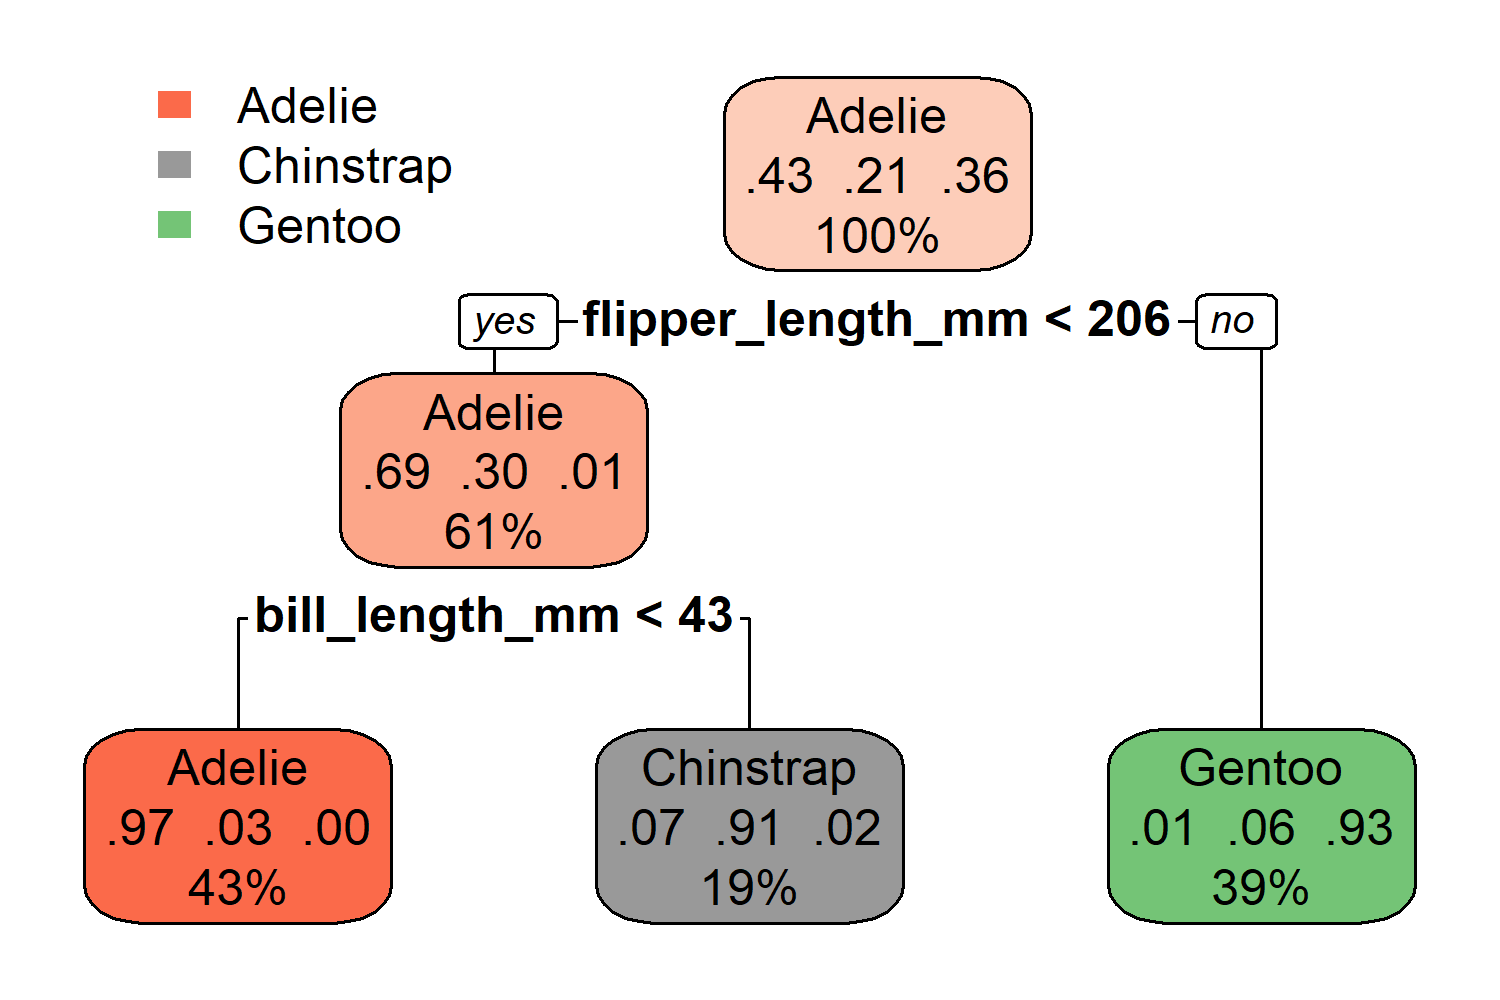
\includegraphics[scale=0.8]{04_decision_tree.png}
    \caption{Decision Tree for Penguin Species}
    \label{fig:my_label}
\end{figure}

This Decision Tree works in the following way. If a penguin has flipper measuring 206mm or more it is classified as a Gentoo penguin. If its flipper measures less than 206mm it is classified in the following manner. As an Adelie penguin if it bill length is less than 43mm or as a Chinstrap penguin it its bill length is 43mm or larger. This very simple algorithm correctly predicted the species of 39 out of 41 Adelie penguins, 19 ou 21 Chinstrap penguins and 35 out of 35 Gentoo penguins present in the testing dataset.

\bibliographystyle{plain}
\bibliography{references.bib}

\end{document}